\section{Setting, contributions, and related works}
\label{2406:sec:main:setting}
\begin{figure}
    \centering
    
    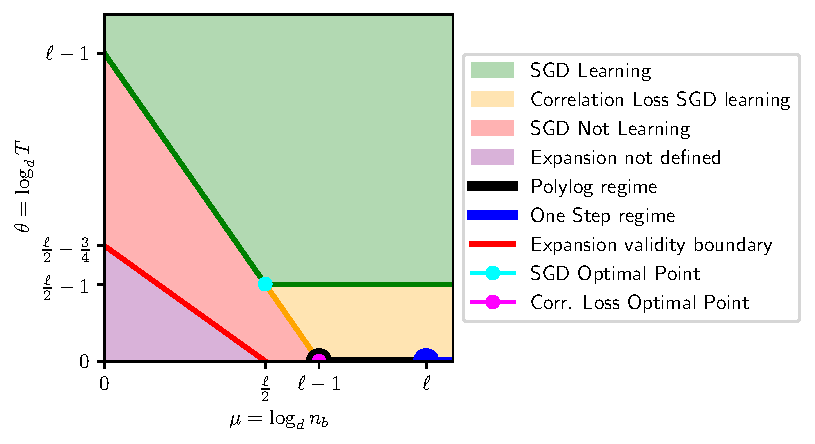
\includegraphics[width=\textwidth]{figs/logT_lognb}
    \caption{\textbf{Time / Batch size tradeoff for weak recovery:} Phase diagram illustrating different SGD learning regimes as a function of the batch size exponent $\mu=\log_d n_b$ and weak recovery time exponent $\theta=\log_d T$. The analysis is dependent on the target's information exponent $\ell$, this particular plot is valid when \(\ell\ge3\). 
    \textbf{\color{notallowedcolor} Not correlating region:} SGD is not able to achieve weak recovery.
    \textbf{\color{noyhatcolor} Self-interaction regime:} SGD is not able to perform weak recovery, but Correlation loss SGD overcomes this limitation.
    \textbf{\color{allowedcolor} Weak recovery region:} SGD successfully achieve weak recovery.
    Note that it exists an \textbf{\color{optimalcolor} optimal choice} at batch size $n_b =O(d^{\sfrac\ell2})$ that minimizes the number of iterations needed by SGD, and another \textbf{\color{magenta} optimal point} at \(n_b=O(d^{\ell-1})\) for \emph{Correlation Loss}.
    The critical line where \(n_b=\Omega(d^{\ell-1})\) is not addressed by our formal. See details about the other two regions (\textbf{\color{black}Poly-log Regime} and \textbf{\color{blue} One-step regime} \citep{dandi2023how}) in Appendix~\ref{2406:app:sec:weakrecoveryglm}.
    }
    \label{2406:fig:cold_start_pd}
\end{figure}

Consider a two-layer neural network with activation function $\sigma$ and first and second layer weights given by $W\in\mathbb{R}^{p\times d}$ and $\vec{a}\in\mathbb{R}^{p}$ respectively:
\begin{align}
\label{2406:eq:main:newtwork_def}
    f(\vec z) = \frac{1}{p} \sum_{j=1}^p a_j \sigma{( \langle \vec z, \vec w_j \rangle)} .
\end{align}
 We are interested in studying the capacity of $f$ to learn from training data $\mathcal{D} = \{(\vec{z}^{\nu}, y^{\nu})_{\nu \in [N]}\in\mathbb{R}^{d+1}\}$.\addnote{In this chapter the input covariate is denoted $\vec z$, playing the role of $\vec x$ in the rest of the thesis.} In the following, we work under the following setting.

\paragraph{Data model ---} As hinted in the introduction, we focus on the case the (noisy) labels depend on the covariates only through a projection over a $k$-dimensional subspace:
\begin{align}
\label{2406:eq:main:teacher_def}
     y^\nu = h^\star(W^\star \vec z^\nu)  + \sqrt{\Delta} \xi^\nu, \quad\vec z^\nu \sim \mathcal{N}(0,I_d) 
\end{align}
where $W^\star = \{\vec w^\star_r\}_{r \in [k]}\in \mathbb{R}^{k \times d}$ are the target weights, $h^\star: \mathbb{R}^k \to \mathbb{R}$ is a non-linear activation function, $\xi^\nu \sim \mathcal{N}(0,1)$ is the label noise with variance given by $\Delta\ge0$. We focus on the case where $k = O(1)$ and $d$ is large, i.e. the label only depends on a few directions of a high-dimensional ambient space. The target function $f^{\star}(\vec{z}) = h^{\star}(W^{\star}\vec{z})$ is often referred to in the literature as a \emph{multi-index model}.

Note that the setting above where we assume a generative model for the data and study the capacity of a model to learn is also known as teacher-student model in the literature. We adopt this terminology and refer to $f^\star$ and $f$ as the \textit{teacher} and the \textit{student} functions, respectively. Similarly, we refer to $W^\star$ and $W$ as the \textit{teacher} and \textit{student} weights.

\paragraph{Hardness of the learning task ---} Characterizing what class of targets are efficiently learned by two-layer networks is arguably one of the key questions in theoretical machine learning. The pivotal work of \cite{arous2021online} provably describes that for $k=1$, the hardness of the learning task is encoded by a single number, the information exponent $\ell$. More precisely, given the activation $h^\star$ in \eqref{2406:eq:main:teacher_def}, $\ell$ is the lowest degree of the Hermite polynomials $\{\mathrm{He}_j\}_{j \in \mathbb N}$ appearing in the Hermite expansion of $h^\star$. This notion generalizes direction-wise for multi-index models ($k>1$), where $\ell$ is known as leap complexity \citep{abbe2023sgd}.

\begin{definition}[Information Exponent \citep{arous2021online}]
\label{2406:def:main:information_exponent}
    \begin{align}
        \ell = \min\{j \in \mathbb{N} : \mathbb{E}_{\xi \sim \mathcal{N}(0,1)}\left[ h^\star(\xi) \mathrm{He}_j(\xi)\right] \neq 0\}
    \end{align}
\end{definition}

\paragraph{Training algorithm ---} Given the training data $\mathcal{D}$, we consider the training of $(W,\vec{a})$ under a \emph{sample splitting} scheme: the data is partitioned $\mathcal{D} = \bigcup_{t=1}^{T}\mathcal{D}_{t}$ into $T =  \left \lfloor \sfrac{N}{n_{b}} \right \rfloor$ disjoint batches $\mathcal{D}_{t}$ of size $n_{b}$, which are used, one every iteration, to train the network.\addnote{This chapter departs from the discrete/continuous time convention of Section~\ref{intro:sec:settings}: here $t$ denotes the discrete SGD step (called $\nu$ there), since $\nu$ is reserved for indexing individual samples within a batch $\mathcal{D}_t$; and, from Section~\ref{2406:sec:main:warm_start} onward, $\tau$ denotes continuous time (called $t$ there).} We consider a common assumption for the training algorithm that is to decouple the training of the hidden weights $W$ and the second layer weights $\vec a$.
By keeping fixed the second layer weights at initialization $\vec a = \vec a_0$, the hidden layer weights $W$ are estimated using (projected) SGD: 
\begin{align}
    \vec w_{j,t+1} =  \frac{\vec{w}_{j,t} - \gamma \nabla_{\vec w_{j,t}}\hat{\mathcal{R}}_t}{\norm{\vec{w}_{j,t} - \gamma \nabla_{\vec w_{j,t}}\hat{\mathcal{R}}_t}} \qquad \forall t \in [T],   \forall j \in [p]
    \label{2406:eq:main:gd_update_weights}
\end{align}
where:
\begin{align} \label{2406:eq:main:projected_sgd}
    \hat{\mathcal{R}}_t = \frac{1}{2n_{b}} \sum_{\nu = 1}^{n_b}(y^\nu-f(\vec z^\nu))^2, \qquad \forall t \in [T]
\end{align}
is the empirical risk over a batch of data. Two comments are in place. First, the gradient at each step is computed using the empirical loss given by fresh, previously, unseen samples coming from $\mathcal{D}_{t}$. Each gradient is thus an unbiased estimator of the true gradient, which means that on average this algorithm minimizes the population risk over $W$:
\begin{align}
\label{2406:eq:main:risk}
        \mathcal R = \mathbb{E}_{(\vec z,y)} \left[\frac12 (y-f(\vec z))^2\right]
\end{align}

Second, the spherical projection allows us to focus just on the direction learned by the network, putting aside the effect of the change of the norm of the weights. Note that in equation \eqref{2406:eq:main:gd_update_weights} we have kept the read-out layer $\vec{a}$ fixed. Optionally, the second layer could also be trained with SGD, as the first layer, or even with the Moore-Penrose pseudo-inverse solution; In this paper, however, we consider it fixed and focus on the \textit{feature learning} step, i.e., the recovery of the low-dimensional space spanned by $W^{\star}$. 


\paragraph{High-dimensional regime ---} We focus on the high-dimensional regime where $d\to\infty$. Of particular interest is the case where the batch size $n_b$ scales with the dimension $d$. Indeed, in modern machine learning, and in particular in the realm of distributed and federated learning, scenarios with large batches, a single pass, and few iterations often become the norm \citep{goyal2017accurate,li2020review} (as for instance when training large language models), further underlining the relevance of this scenario.

More precisely, we assume a scaling of the relevant parameters, i.e., learning rate and the batch size, with \(d\), as follows
\begin{equation}\label{2406:eq:main:gamma_nb_scalings}
\gamma = \gamma_0 d^{-\delta} \quad\text{and}\quad n_b = n_0 d^\mu,
\end{equation}
with \(\mu \ge 0\) and \(\delta\) could possibly be any real value. The exponents $(\delta, \mu)$ characterize the Time / Complexity tradeoff illustrated in the phase diagram (Figure~\ref{2406:fig:cold_start_pd}). More precisely, the figure shows the time complexity $T = T_0 d^{\theta}$ as a function of the batch size exponent $\mu$. The time exponent $(\theta)$ is linked to the learning-rate exponent $(\delta)$ and the information exponent $(\ell)$, and determining this relation is the main object of analysis of the following sections.  

\paragraph{Weak recovery of the target ---} The central object of our analysis is to characterize the time iterations needed for the SGD dynamics defined in Equation~\eqref{2406:eq:main:projected_sgd} to learn the low-dimensional features $W^\star$. More precisely, we are interested in studying the number of steps to achieve order one correlation with the target weights $W^\star$. We refer to this condition as \textit{weak recovery} of the target subspace, formalized in the following definition.
\begin{definition}[Weak recovery]
\label{2406:def:weak_recovery}
    The \textit{target subspace} $V^\star$ is defined as the span of the rows of the target weights $W^\star$:
    \begin{align}
    \label{2406:eq:main:teacher_subspace_def}
        V^\star = {\rm span}(\vec w^\star_1, \dots, \vec w^\star_k)
    \end{align}
    We define the following weak recovery stopping time for a parameter $\eta \in (0,1)$ independent from $d$:
\begin{equation}
    t^{+}_{\eta} = \min\{t \geq 0: \lVert W W^{\star \top} \rVert_F \geq \eta\}
\end{equation}
\end{definition}

Our key objective is to characterize the largest affordable batch size $n_b$ to achieve weak recovery of the relevant target subspace $V^\star$ while minimizing the training time iterations $T$. Indeed, the updates of one-pass SGD in Equation~\eqref{2406:eq:main:projected_sgd} consist of sums of independent terms that can be parallelized efficiently with decentralized learning protocols.

Our \textbf{main contributions} in this paper are the following:
\begin{itemize}
    \item We study how the batch size influences the number of steps required to learn a target function, for different information exponents of the problem. We introduce a schematic phase diagram describing the different learning regimes, see Figure~\ref{2406:fig:cold_start_pd}. 
    
    \item We show that performing gradient updates with large batch sizes can reduce the training time without changing the total sample complexity to weakly recover the teacher subspace only up to \(n_b \lesssim d^{\sfrac{\ell}{2}}\) samples per step, with \(d\) the data dimension and $\ell$ the information exponent of the target. Beyond this limit, larger batch sizes are detrimental for one-pass SGD.
    
     \item We characterize that it is possible to improve over this fundamental limitation of one-pass SGD by using gradient updates on the correlation loss, namely  \textit{Correlation loss SGD}. We provably show that the number of steps needed to weakly correlate with the target with this new training protocol can then be pushed down to \(T=\mathrm{polylog}(d)\) when using batch sizes $n_b = O(d^{\ell -1})$, with $\ell$ the information exponent.
     Additionally, we provide sharp prescription on how to scale the learning rate with batch size and input dimension, in order to achieve the best time-memory tradeoff.
     
    \item We show that the asymptotic training dynamics is described by a system of Ordinary Differential Equations (ODEs) that can be solved exactly. We leverage on the ODE description to characterize the different learning phases of two-layer networks when initialized with non-vanishing initial correlation with the target direction to be learned (warm starts). Furthermore, we also discuss finite \(d\) corrections to the asymptotic dimension-free description. 
    
    \item Finally, we validate and illustrate our theoretical results with numerical experiments.
\end{itemize}

The code to reproduce representative figures is available in our \href{https://github.com/IdePHICS/batch-size-time-complexity-tradeoffs}{GitHub~repository}. We refer to Appendix~\ref{2406:sec:app:hyperparams} for details on the numerical implementations while the rigorous proofs of the main results are detailed in Appendix~\ref{2406:sec:app:proofs}. 

\paragraph{Other related works ---} 
The dynamics of Stochastic Gradient Descent (SGD) in two-layer neural networks, particularly when trained on synthetic Gaussian data, have been a topic of interest since the seminal works in the mid-1990s \cite{saad1995line,saad1996dynamics,biehl1995learning,riegler1995line}. This area has experienced a resurgence in recent years \cite{tan2019online,goldt2019dynamics,veiga2022phase,arnaboldi2023high,arnaboldi2024escaping,berthier2023learning,arous2021online,paquette2022homogenization,collinswoodfin2023hitting,martin2024impact}.

Many theoretical efforts highlighted the class of functions that are efficiently learned by two layer neural networks. In the context of single-index targets, \cite{arous2021online} introduces the notion of information exponent to quantify the hardness of the learning task. Similarly, for multi-index models,  
\citep{abbe2022merged,abbe2023sgd}, building on their earlier work \citep{abbe2021staircase},
demonstrated how the leap complexity of target functions dictates the amount of training samples needed from two-layer networks in the mean-field limit to learn the target. Note that \cite{abbe2023sgd} also considered the case of $n_b \lesssim O(d)$. Numerous theoretical studies devoted to the understanding of the feature learning regime in two-layer networks often assume an asymptotically vanishing initialization for the second layer weights $\vec a_0$ in Equation~\eqref{2406:eq:main:newtwork_def}, see e.g. \citep{abbe2022merged,berthier2023learning,abbe2023sgd}. Although this assumption is amenable for theoretical characterizations, our analysis provably shows that a careful reasoning on the second layer magnitude is needed to offer a complete portrait of the learning dynamics of SGD. More precisely, we describe a sharp divergence when the batch size $n_b \gg d^{\sfrac{\ell}{2}}$ between the dynamics of SGD when optimizing the MSE loss (vanilla SGD), in contrast to the correlation loss $\Tilde{\ell} = \frac{1}{n_b}\sum_{\nu \in [n_b]} 1-y^{\nu}f(\vec z^{\nu})$ (Correlation loss SGD). The latter training protocol is indeed equivalent to consider an asymptotically vanishing second layer weights $\vec a_0$ at initialization in the optimization routine, e.g. see 
\citep{damian2023smoothing}. 



Closer to us, the analysis of the {\it first} gradient descent step with large $n_b$ has been discussed in detail in recent papers \citep{ba2022high,damian2022neural,dandi2023how}. \cite{ba2022high} showed that a single large learning rate gradient step allows beating kernel methods when the number of training samples is proportional to the input dimension. While their results are limited to single-index target and to a single gradient step, \cite{damian2022neural} further showed that with $n = \omega(d^2)$ samples, two-layer nets can learn multi-index target function with zero first Hermite coefficient ($\ell$=2). \cite{dandi2023how} extended their conditions on the sample complexity to general $\ell\geq 1$, showed this complexity is optimal for single-step learning, and extended the results to higher information exponents. Although motivated from different objectives,  \cite{sclocchi2024different} heuristically sketch a phase diagram for the performance of SGD on realistic datasets as a function of the algorithm's relevant parameters, i.e. batch size and learning rate. 


A common assumption in  theoretical studies is to consider
sample-splitting schemes for the training protocol.  At each iteration, the optimization algorithm is run using a fresh batch of observations of the model, drawn independently of past iterations; this routine has been used extensively in the analysis of iterative algorithms (see e.g. \citep{chandrasekher2021sharp,jain2013low,hardt2014fast,jain2015fast,kwon2019global}).
